\documentclass[a4paper, twoside, 12pt]{article}
\usepackage{outline}
\usepackage{pmgraph}
\usepackage[normalem]{ulem}
\usepackage{amsmath}
\usepackage{listings}
\usepackage{lipsum}
\usepackage{layout}
\usepackage{indentfirst}
\usepackage[brazilian]{babel}
\usepackage{float}
\usepackage[utf8]{inputenc}
\usepackage[T1]{fontenc}
\usepackage{lingmacros}
\usepackage{tree-dvips}
\usepackage{multirow}
\usepackage{caption}
\usepackage{subcaption}
\usepackage{titlesec}
\usepackage{chngcntr}
\usepackage{indentfirst}
\usepackage{hyperref}

% Images
\usepackage{graphicx}
\usepackage{txfonts}
\usepackage{graphics}


% \setcounter{secnumdepth}{5}

\titleformat{\paragraph}
{\normalfont\normalsize\bfseries}{\theparagraph}{1em}{}
\titlespacing*{\paragraph}
{0pt}{3.25ex plus 1ex minus .2ex}{1.5ex plus .2ex}

\numberwithin{equation}{section}

\title{\textbf{CC299 - Projeto 04}}
\author{Leonardo M. M. de O. Carvalho}
\date{\oldstylenums{00}/\oldstylenums{00}/\oldstylenums{00}}

%--------------------Make usable space all of page
\setlength{\oddsidemargin}{0in}
\setlength{\evensidemargin}{0in}
\setlength{\topmargin}{0in}
\setlength{\headsep}{-.25in}
\setlength{\textwidth}{6.5in}
\setlength{\textheight}{8.5in}
\counterwithin{paragraph}{subsubsection}

%--------------------Indention
\setlength{\parindent}{1cm}

\begin{document}
\bibliographystyle{plain}
%--------------------Title Page
\maketitle
\tableofcontents
 
%--------------------Begin sections
\begin{abstract}
    \textit{Este relatório tem dois objetivos. O primeiro é apresentar, de forma breve, a formulação do esquema TVD de Harten, Yee e Warming \cite{YEE_NASATM_1983}. O segundo é, de forma mais aprofundada, apresentar os resultados obtidos pela versão explícita do esquema em primeira ordem. Na primeira seção será apresentada a formulação do fluxo modificado obtido com o esquema. Para manter o relatório mais conciso, apenas a formulação referente a coordenada espacial x e o método de marcha no tempo foram documentados. Na seção de resultados são apresentados os contornos de pressão e densidade obtidos com diferentes malhas, comparações gráficas entre os resultados numéricos e analíticos e um estudo de desempenho do código variando o refinamento global da malha. A seção de conclusões será responsável por discutir a formulação e os resultados apresentados nas outras seções do relatório.}
\end{abstract}

\section{Esquema de Harten - Formulação}
Nesta seção será documentada a formulaçao do esquema de Harten, Yee e Warming \cite{YEE_JCP_1985} aplicado às equações de Euler bidimensionais em coordenadas cartesianas. Deve-se ter em mente que a notação usada mantem alinhamento com a proposta no paper \cite{YEE_NASATM_1983} onde o método é apresentado. Dito isso, podemos apresentar as equações de Euler em duas dimensões como:
\begin{equation}
\frac{\partial U}{\partial t}+\frac{\partial F(U)}{\partial x}+\frac{\partial G(U)}{\partial y}=0.
\end{equation}
Onde os vetores de propriedades podem ser definidos como:
\begin{equation}
U=\begin{Bmatrix} \rho \\  m\\ n\\ e \end{Bmatrix},\:F(U)=\begin{Bmatrix} m\\ \frac{m^{2}{\rho}}+p\\ mv\\ (e+p)\frac{m}{\rho} \end{Bmatrix}, \: G(U)=\begin{Bmatrix}
n\\ 
nu\\ 
\frac{n^{2}}{\rho}+p\\ 
(e+p)\frac{n}{\rho}
\end{Bmatrix}.
\end{equation}
Nesse caso $m=\rho u$ e $n=\rho v$. Deve-se ainda definir $\rho$ como a massa específica do fluído, $u$ e $v$ como as componentes de velocidade do escoamento, $e$ como energia total por unidade de volume e $p$ como pressão. A pressão por sua vez pode ser calculada usando-se:
\begin{equation}
p=(\gamma-1)\left [ e-\frac{(m^{2}+n^{2})}{2\rho} \right ].
\end{equation}
Onde nesse caso, $\gamma$ representa a razão de calores específicos ($1.4$ para o ar).

Considerando que $A=\frac{\partial F(U)}{\partial U}$ é a jacobiana das equações de Euler para o vetor de fluxos na direção $x$. Define-se os autovalores de $A$ como:

\begin{equation}
\left ( a^{1}_x,a^{2}_x,a^{3}_x,a^{4}_x \right )=\left ( u-c,u,u+c,u \right ).
\end{equation}
Onde $c$ é a velocidade do som local. Mais ainda, podemos definir os autovetores pela direita na forma de matrizes $R_{x}=\left (R_{x}^{1},R_{x}^{2},R_{x}^{3},R_{x}^{4}  \right )$ como :
\begin{equation}
R_{x}=\begin{bmatrix}
1    & 1               & 1    & 0\\ 
u-c  & u               & u+c  & 0\\ 
v    & v               & v    & 1\\ 
H-uc & (u^{2}+v^{2})/2 & H+uc & v
\end{bmatrix}
\end{equation}
e
\begin{equation}
H=\frac{c^{2}}{\gamma-1}+\frac{u^{2}+v^{2}}{2}.
\end{equation}

Considerando a matriz $R_{x}$, pode-se definir sua inversa como:
\begin{equation}
R^{-1}_{x}=\begin{bmatrix}
0.5(b_{1}+u/c) & 0.5(-b_{2}u-1/c) & 0.5(-b_{2}v) & 0.5b_{2} \\ 
1-b_{1}        & b_{2}u           & (b_{2}v)     & -b_{2}\\ 
0.5(b_{1}-u/c) & 0.5(-b_{2}u+1/c) & 0.5(-b_{2}v) & 0.5b_{2}\\ 
-v             & 0                & 1            & 
0\end{bmatrix},
\end{equation}
sendo
\begin{equation}
b_{1}=b_{2}\frac{(u^{2}+v^{2})}{2}
\end{equation}
\begin{equation}
b_{1}=\frac{\gamma-1}{c^{2}}.
\end{equation}
Obedecendo um espaçamento uniforme entre os pontos da malha, define-se o vetor $\alpha$ como sendo:
\begin{equation}
\begin{bmatrix}
\alpha^{1}_{j+1/2}\\ 
\alpha^{2}_{j+1/2}\\ 
\alpha^{3}_{j+1/2}\\ 
\alpha^{4}_{j+1/2}
\end{bmatrix}=
\begin{bmatrix}
0.5(aa-bb)\\ 
\Delta_{j+1/2}\rho\\ 
0.5(aa+bb)\\ 
\Delta_{j+1/2}n-v_{j+1/2}\Delta_{j+1/2}\rho
\end{bmatrix}
\end{equation}
onde
\begin{equation}
aa=\frac{\gamma-1}{c^{2}_{j+1/2}}\left [ \Delta_{j+1/2}e+\frac{u^{2}_{j+1/2}+v^{2}_{j+1/2}}{2}\Delta_{j+1/2}\rho-u_{j+1/2}\Delta_{j+1/2}m-v_{j+1/2}\Delta_{j+1/2}n \right ]
\end{equation}
\begin{equation}
bb=\left [ \Delta_{j+1/2}m-u_{j+1/2}\Delta_{j+1/2}\rho \right ]/c_{j+1/2}.
\end{equation}
O operador de salto $\Delta_{j+1/2,k}[]$ é :

\begin{equation}
    \Delta_{j+1/2,k}=[]_{j+1,k} - []_{j,k}
\end{equation}

A definição para a coordenada $y$ é análoga à feita até agora para a direção $x$ e esta detalhadamente definida em \cite{YEE_NASATM_1983}. Com isso, devemos agora finalizar a definição teórica e definir o fluxo modificado como:
\begin{equation}
\bar{F}^{n}_{j+1/2,k}=\frac{1}{2}\left [ F(U_{j,k})+F(U_{j+1,k}) \right ]+\frac{1}{2}\sum_{l=1}^{4}\left [g^{l}_{j}+g^{l}_{j+1}-Q(a^{l}_{j+1/2}+\gamma_{j+1/2}^{l})\alpha^{l}_{j+1/2}  \right ]R^{l}_{j+1/2}.
\end{equation}
Neste ponto é prudente avisar o leitor que o vetor $g^{l}_{j+1}$ seria responsável por aumentar a ordem do esquema \cite{YEE_NASATM_1983}. Como apenas o esquema de primeira ordem foi implementado, esse vetor não será definido aqui. Na equação 1.14, a função $Q(z)$ pode ser definida como:
\begin{equation}
Q(z)=\begin{cases} 
\frac{1}{2}\left ( \frac{z^{2}}{\delta}+\delta \right ), \: |z| <\delta\\
|z|,\: |z|\geq \delta
\end{cases}.
\end{equation}

Por último, para fazer a marcha no tempo das propriedades, usa-se o seguinte esquema proposto, em \cite{YEE_NASATM_1983}.
\begin{equation}
U^{*}_{j,k}=U^{n}_{j,k}-\frac{\Delta t}{\Delta x}\left ( \bar{F}^{n}_{j+1/2,k}-\bar{F}^{n}_{j-1/2,k} \right )=L_{x}U^{n}_{j,k}
\end{equation}
\begin{equation}
U^{n+1}_{j,k}=U^{*}_{j,k}-\frac{\Delta t}{\Delta x}\left ( \bar{G}^{n}_{j+1/2,k}-\bar{G}^{n}_{j-1/2,k} \right )=L_{x}U^{*}_{j,k}.
\end{equation}
De forma mais concisa, podemos definir a marcha no tempo como:
\begin{equation}
U_{j,k}^{n+1}=L_{y}L_{x}U^{n}_{j,k}.
\end{equation}

Neste ponto, finaliza-se todas as definições necessárias para a implementação do esquema. Na próxima seção serão apresentados os resultados obtidos com o código.


\section{Resultados e discussões}
Nesta seção serão apresentados alguns resultados referentes ao problema simplificado da reflexão de um choque oblíquo. Esse problema é composto por um choque com ângulo do choque em relação a placa plana superior de 29 graus. Essa onda de choque reflete sobre uma placa plana e continua até a saída do domínio. Uma esquematização do problema está disponível na proposta do trabalho \cite{AZEVEDO}.
        \begin{figure}[htb]
            \centering
            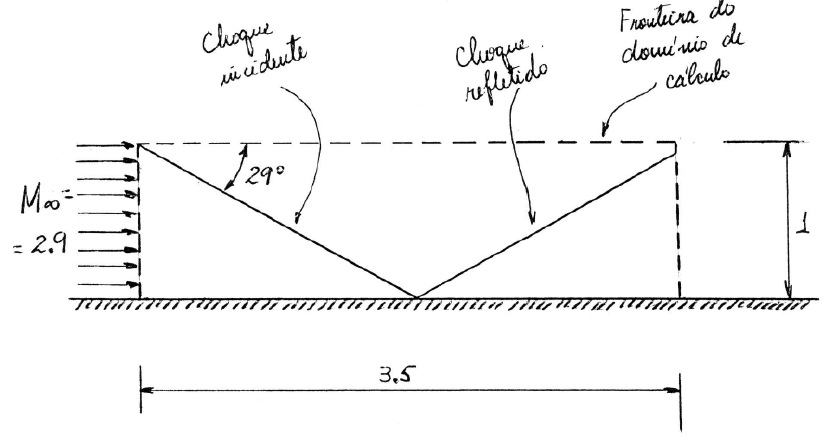
\includegraphics[width=.7\linewidth,height=50mm]{pics/shock.png}
            \caption{Esquematização do problema resolvido \cite{AZEVEDO}}
            \vspace*{-5pt}
        \end{figure}
Para resolver esse problema, foi usada uma malha cartesiana composta por pontos igualmente espaçados. As equações descritas na seção anterior foram resolvidas utilizando-se diferenças finitas. O código final exige do usuário apenas parâmetros básicos tais como: Tamanho do passo no tempo, número de passos e número de pontos em cada direção espacial. O código foi feito utilizando-se linguagem FORTRAN 90 com extensivo uso de alocação dinâmica de memória. O uso da alocação dinâmica facilitou os estudos de refinamento.

    \subsection{Malhas usadas}
        \begin{figure}[H]

        \begin{subfigure}{.5\textwidth}
        \centering
        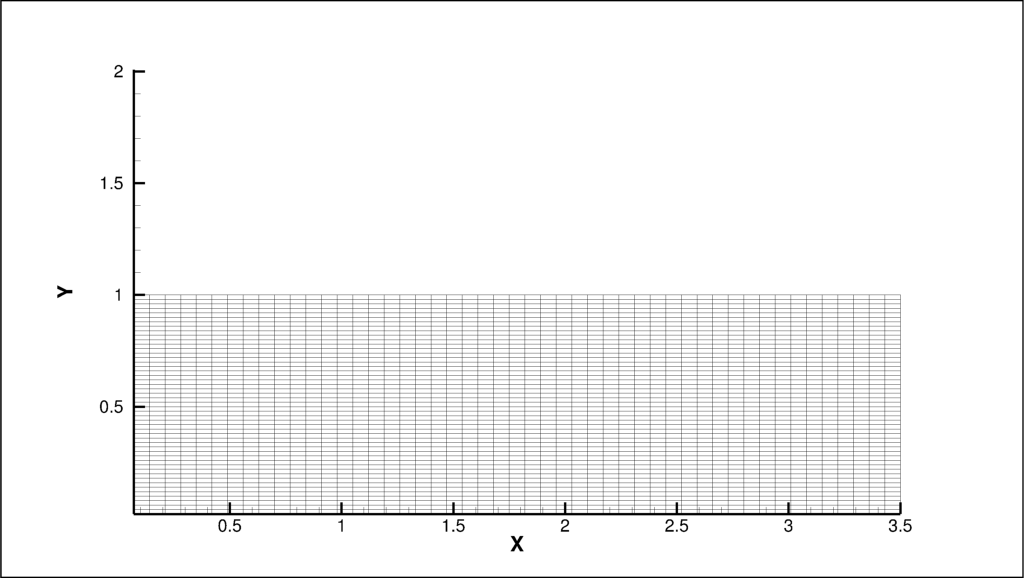
\includegraphics[width=.9\linewidth]{pics/mesh_5050.png}
        \caption{Malha com $50x50$ pontos}
        \label{fig:sfig1}
        \end{subfigure}%
        \begin{subfigure}{.5\textwidth}
        \centering
        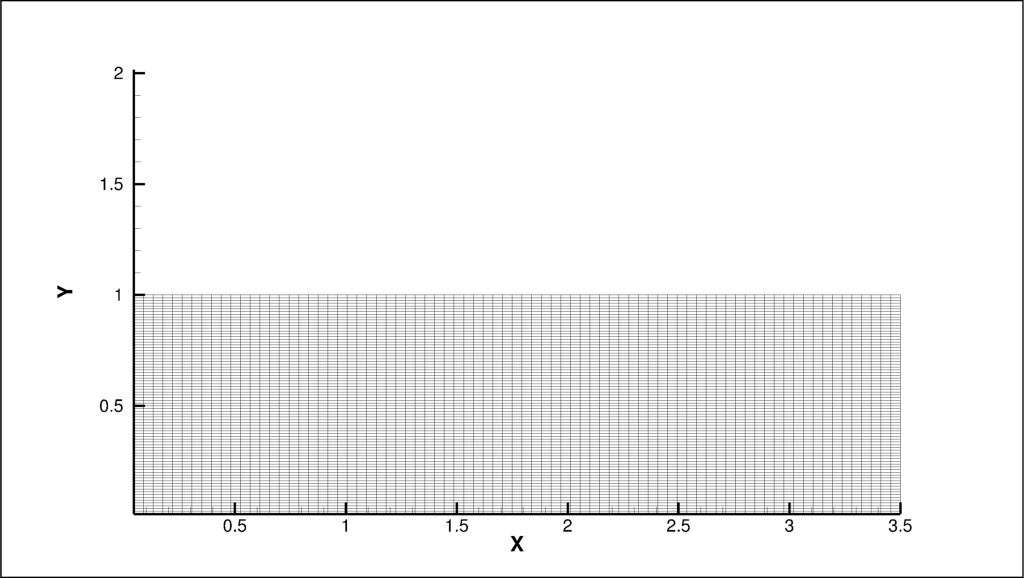
\includegraphics[width=.9\linewidth]{pics/mesh_8080.png}
        \caption{Malha com $80x80$ pontos}
        \label{fig:sfig2}
        \end{subfigure}
        \\
        \begin{subfigure}{.5\textwidth}
        \centering
        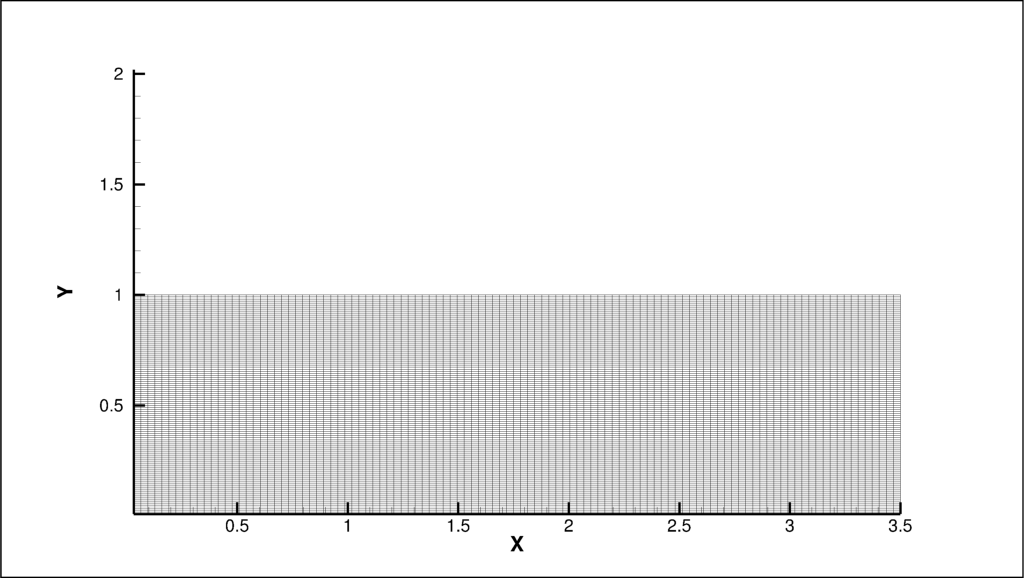
\includegraphics[width=.9\linewidth]{pics/mesh_110110.png}
        \caption{Malha com $110x110$ pontos}
        \label{fig:sfig1}
        \end{subfigure}%
        \begin{subfigure}{.5\textwidth}
        \centering
        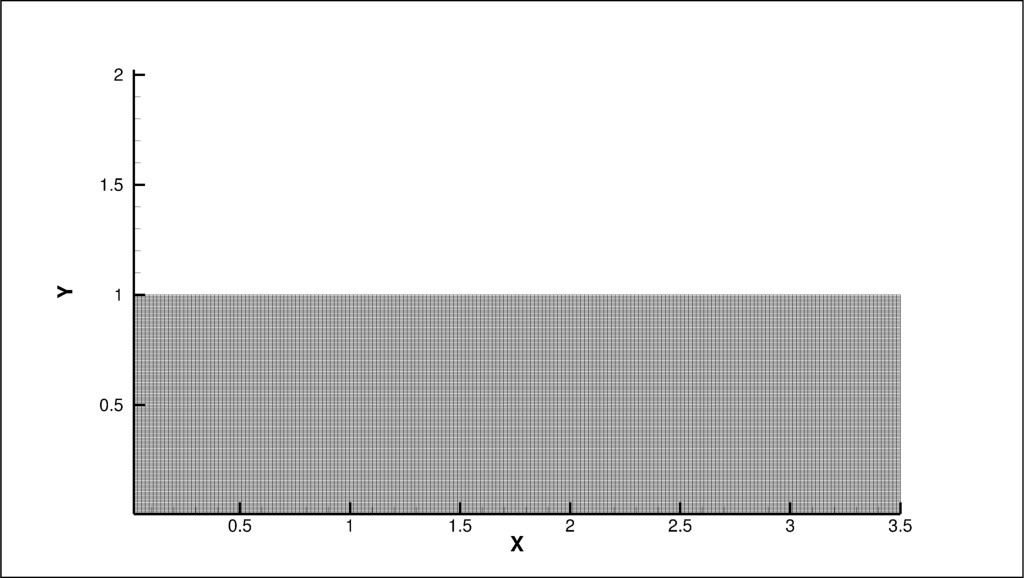
\includegraphics[width=.9\linewidth]{pics/mesh_200200.png}
        \caption{Malha com $200x200$ pontos}
        \label{fig:sfig2}
        \end{subfigure}

        \caption{Malhas usadas durante os cálculos.}
        \label{fig:fig}
        \vspace*{-5pt}
        \end{figure}

    \subsection{Desempenho computacional e numérico}
Nesta seção serão apresentados os resultados referentes ao desempenho numérico e às comparações com a solução analítica.
        \begin{figure}[H]
            \centering
            \includegraphics[width=.9\linewidth]{pics/residues.pdf}
            \caption{Comparação entre os resíduos.}
            \vspace*{-5pt}
        \end{figure}

        \begin{figure}[H]
            \centering
            \includegraphics[width=.9\linewidth]{pics/pressures.pdf}
            \caption{Comparação entre as distribuições de pressão em $y=0.5$}
            \vspace*{-5pt}
        \end{figure}

        \begin{figure}[htb]
            \centering
                \includegraphics[width=.8\linewidth]{pics/comp_time.pdf}
            \caption{Comparação entre os tempos por iteração com o aumento do número de pontos.}
            \vspace*{-5pt}
        \end{figure}

    \subsection{Contornos}
    Nesta seção serão apresentados os contornos gerados pelo código. Quanto aos contornos de pressão, os valores esperados estão esquematizados na figura 6.
        \begin{figure}[H]
            \centering
            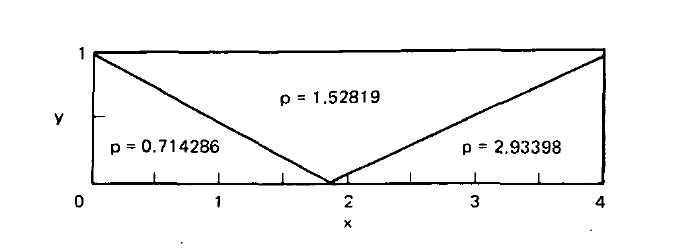
\includegraphics[width=.9\linewidth]{pics/results.png}
            \caption{Valores esperados de pressão para os contornos de pressão.\cite{YEE_NASATM_1983}}
            \vspace*{-5pt}
        \end{figure}
        \begin{figure}[H]

            \begin{subfigure}{.5\textwidth}
            \centering
            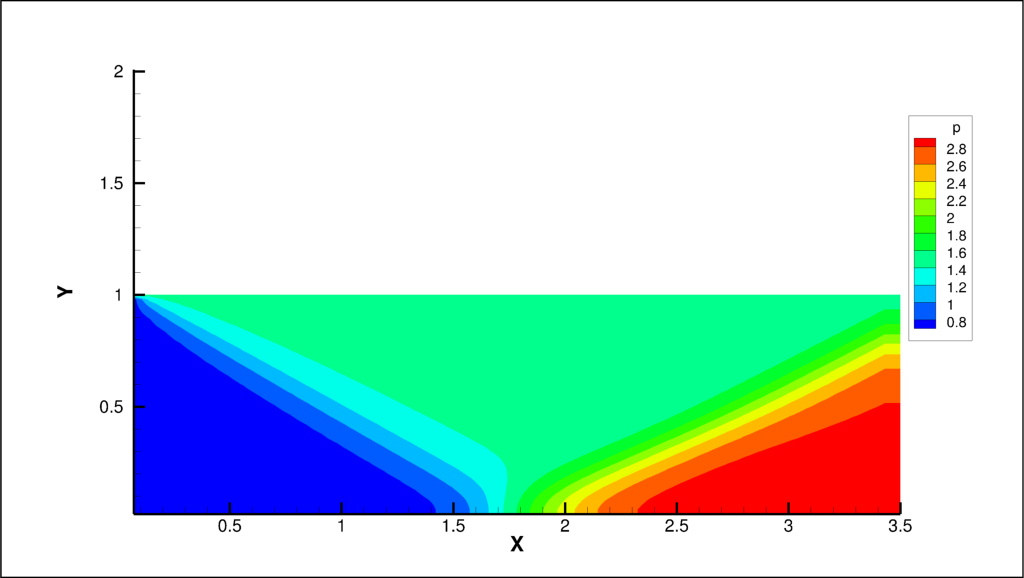
\includegraphics[width=.9\linewidth]{pics/pressure_5050.png}
            \caption{Malha com $50x50$ pontos}
            \label{fig:sfig1}
            \end{subfigure}%
            \begin{subfigure}{.5\textwidth}
            \centering
            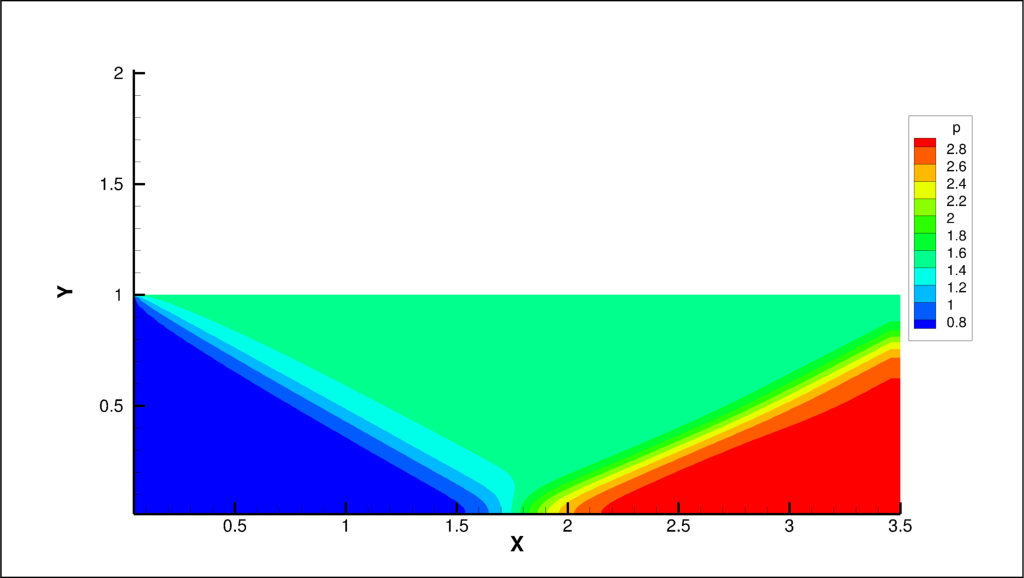
\includegraphics[width=.9\linewidth]{pics/pressure_8080.png}
            \caption{Malha com $80x80$ pontos}
            \label{fig:sfig2}
            \end{subfigure}
            \\
            \begin{subfigure}{.5\textwidth}
            \centering
            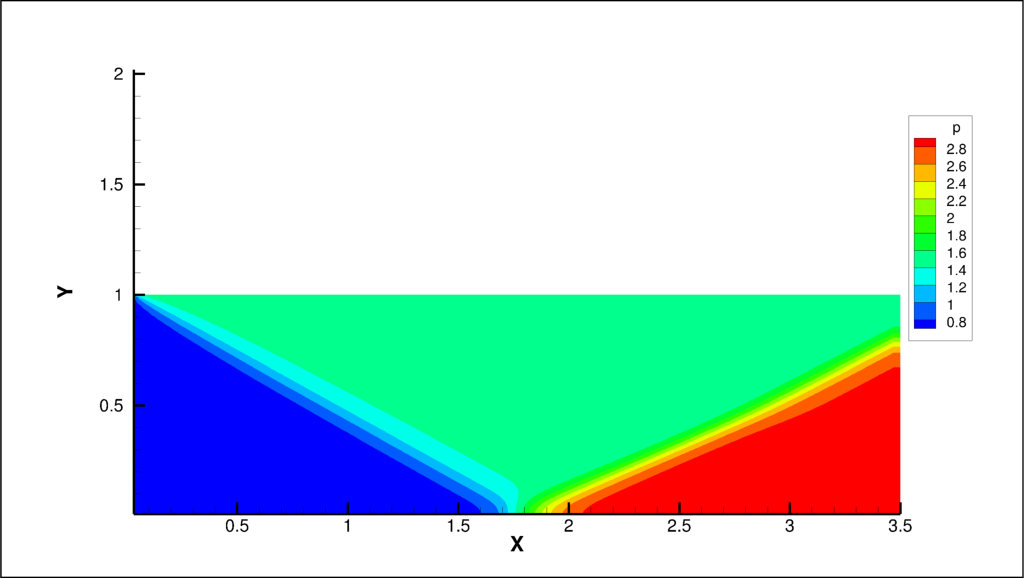
\includegraphics[width=.9\linewidth]{pics/pressure_110110.png}
            \caption{Malha com $110x110$ pontos}
            \label{fig:sfig1}
            \end{subfigure}%
            \begin{subfigure}{.5\textwidth}
            \centering
            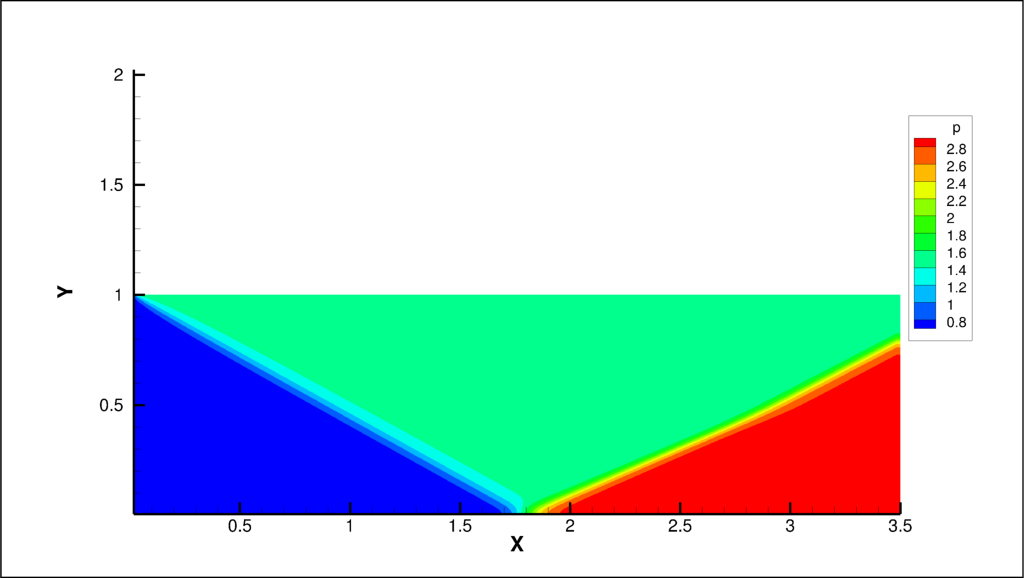
\includegraphics[width=.9\linewidth]{pics/pressure_200200.png}
            \caption{Malha com $200x200$ pontos}
            \label{fig:sfig2}
            \end{subfigure}

        \caption{Contornos de pressão adimensionalizada.}
        \vspace*{-5pt}
        \label{fig:fig}
        \end{figure}

        \begin{figure}[H]

            \begin{subfigure}{.5\textwidth}
            \centering
            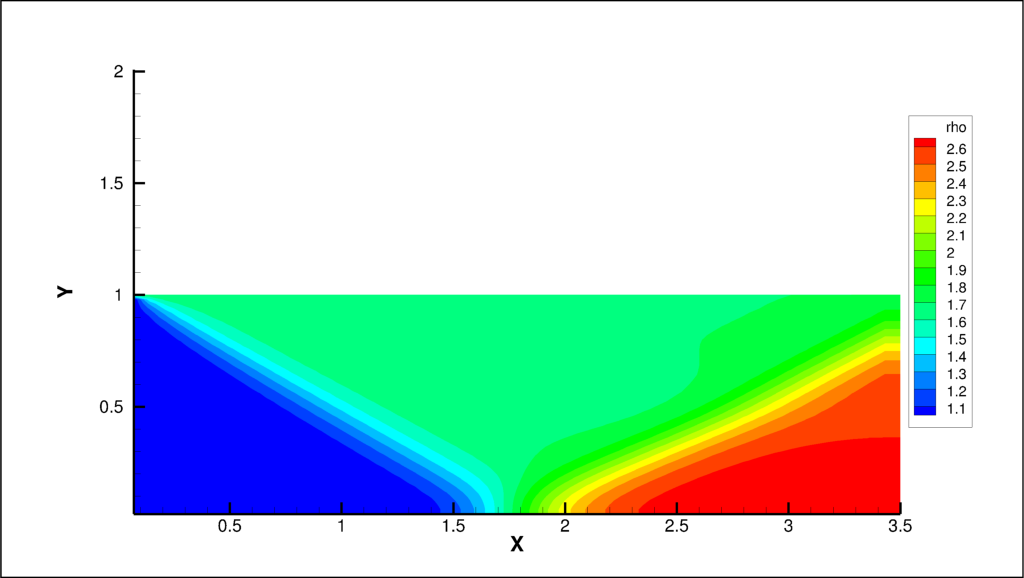
\includegraphics[width=.9\linewidth]{pics/rho_5050.png}
            \caption{Malha com $50x50$ pontos}
            \label{fig:sfig1}
            \end{subfigure}%
            \begin{subfigure}{.5\textwidth}
            \centering
            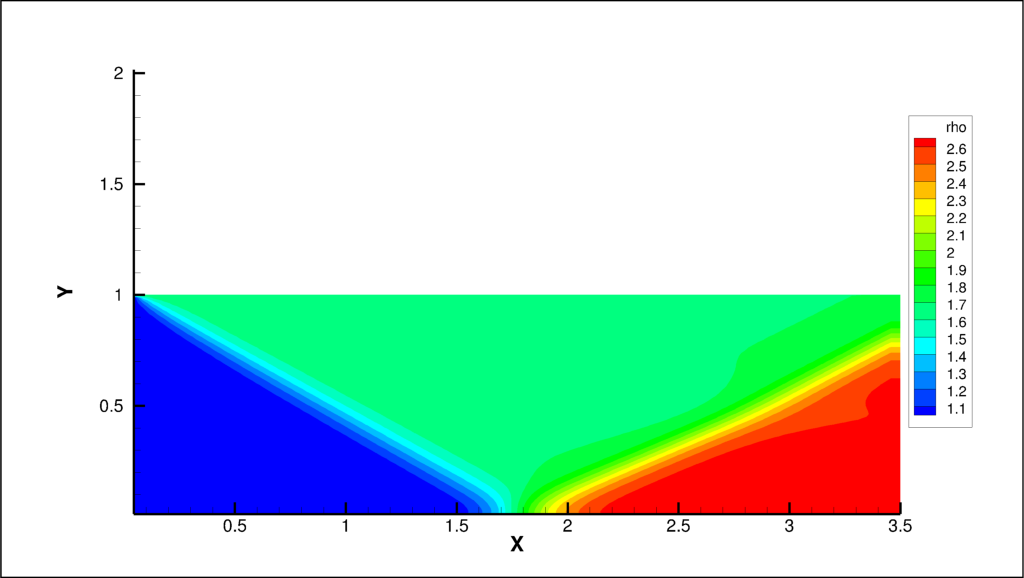
\includegraphics[width=.9\linewidth]{pics/rho_8080.png}
            \caption{Malha com $80x80$ pontos}
            \label{fig:sfig2}
            \end{subfigure}
            \\
            \begin{subfigure}{.5\textwidth}
            \centering
            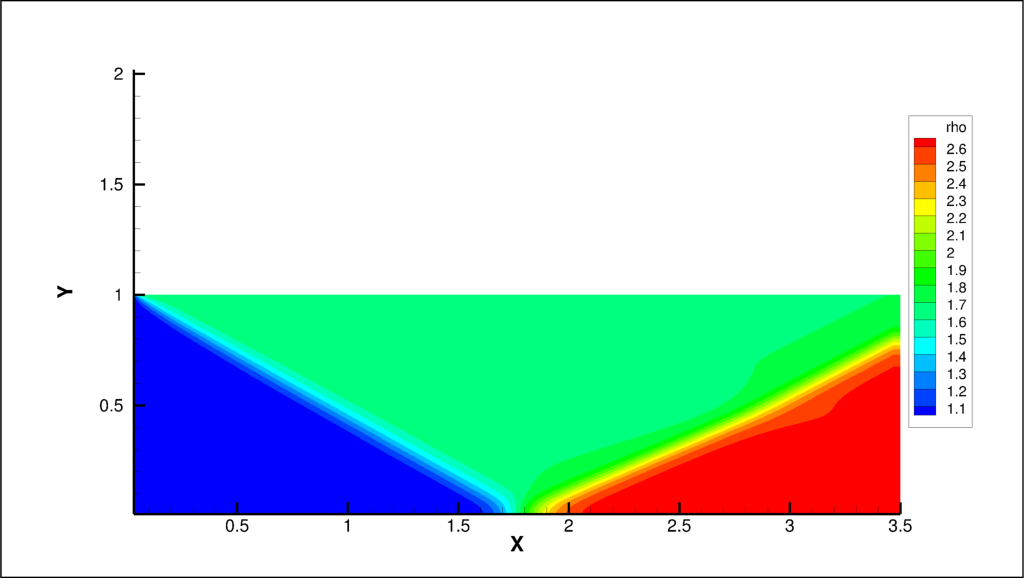
\includegraphics[width=.9\linewidth]{pics/rho_110110.png}
            \caption{Malha com $110x110$ pontos}
            \label{fig:sfig1}
            \end{subfigure}%
            \begin{subfigure}{.5\textwidth}
            \centering
            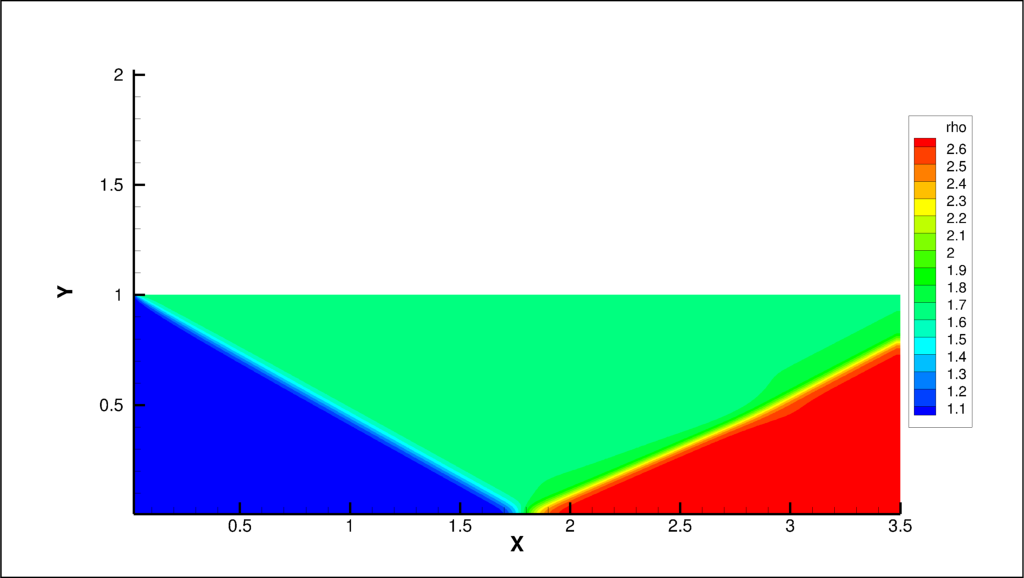
\includegraphics[width=.9\linewidth]{pics/rho_200200.png}
            \caption{Malha com $200x200$ pontos}
            \label{fig:sfig2}
            \end{subfigure}

        \caption{Contornos de densidade adimensionalizada.}
        \label{fig:fig}
        \vspace*{-5pt}
        \end{figure}


\section{Conclusões}
Baseando-se na formulação apresentada e implementada, é possível concluir que o código resultou em uma solução aceitável. Diz-se aceitável pois, as comparações com os resultados analíticos não conseguem atingir os patamares esperados entre os choques. Porém, observando os contornos de forma qualitativa e seu comportamento com o refinamento da malha, pode-se dizer que o esquema está implementado de forma correta. 

Computacionalmente o código parece ter um comportamento coerente com o aumento da malha. No entanto, melhorias significativas poderiam ser feitas usando-se de forma mais inteligente os vetores necessários pelo método. A inteligência do uso, nesse caso, estaria em acessar os indices na mesma forma que o FORTRAN guarda as matrizes. O uso de alocação dinâmico também poderia ser modificado e levado todo para o programa principal. O fato de algumas alocações ainda estarem sendo feitas dentro das subrotinas, dificulta otimizações visto que o processo de alocação de memória é pouco otimizável.

O código deste projeto está disponível em: \href{https://github.com/lmarmotta/n.cfd_oblique.shock2d}{link para o código}

\bibliography{refs.bib}

\end{document}

